% BOTH

Hauptziel der Arbeit war es die Komponenten gut zu vermessen und ihre Leistung zu verifizieren.

\subsubsection*{Setup}
TODO:

\subsubsection*{Software}
TODO:

\subsubsection*{Erste Messungen}

Mit einer ersten bestückten Leiterplatte wurden daher mit dem Oszilloskop erste Messungten durchgeführt, welche eine generelle Funktionstüchtigkeit bezeugten, welche aber gar nicht zufriedenstellend war.

\begin{figure}[H]
\begin{center}
    \includegraphics[width=0.9\textwidth]{data/images/messungen/erste_messung}
    \caption{Erste Messungen des Gesamtsystems. Inkorrekt terminiert. Mit Oszilloskop gemessen.}
    \label{fig:messungen_erste}
\end{center}
\end{figure}

Diese Kurve sieht wahnsinnig unschön aus. Gerade bei den Peaks gibt es fiese Ausreisser. Und was ebenfalls nicht zu vernachlässigen ist, sind die 180 Grad Phasenverschiebung.
Auch sieht man hier, dass der dass der Input des Funktionsgenerators ziemlich viel Rauschen hat, welches sich auch in Grafik \ref{fig:messungen_zweite} zeigt.
Dort sieht man gut, dass der Input ziemlich rauscht. Deswegen haben wir versucht N und P voneinander zu subtrahieren. Und so das Rauschen zu eliminieren. Dies hat sogar relativ gut geklappt. Dies ist natürlich nicht ganz sauber, ging aber für eine erste Verifikation sehr gut.

\begin{figure}[H]
\begin{center}
    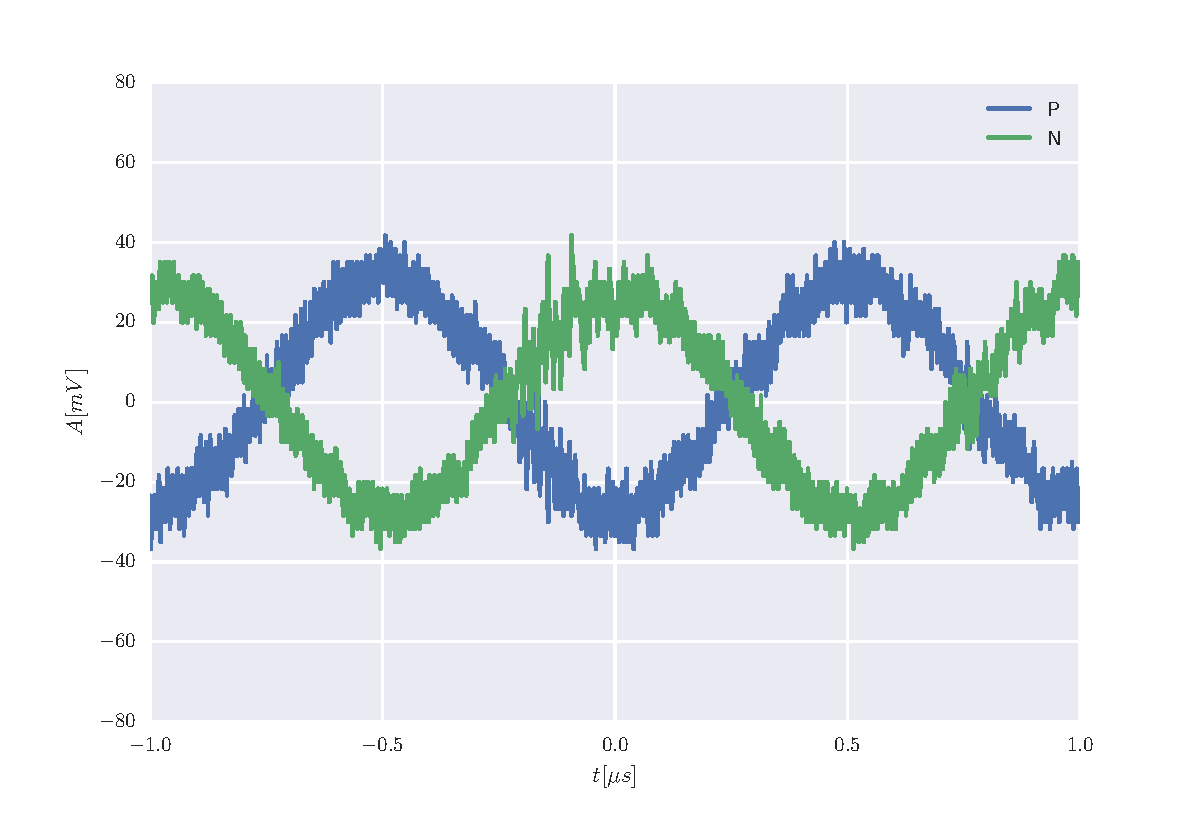
\includegraphics[width=0.9\textwidth]{data/images/messungen/zweite_messung_NP}
    \includegraphics[width=0.9\textwidth]{data/images/messungen/zweite_messung_INOUT}
    \caption{Erste Messungen des Gesamtsystems. Inkorrekt terminiert. Mit Oszilloskop gemessen.}
    \label{fig:messungen_zweite}
\end{center}
\end{figure}

Bei diesen Messungen war jedoch das DUT nicht korrekt terminiert. Dies war einer der Knackpunkte zum Anfang. Es war uns bekannt, dass Dinge in diesem Gebiet korrekt terminiert werden müssen. Wenn das DUT nicht korrekt belastet wird können ungewollte Effekte auftreten. Deswegen sind diese ersten Messungen mit Vorsicht zu geniessen und dürfen nur als Anhaltspunkt und nicht als exakte Messung genommen werden.

Eigentlich wären zur korrekten Terminierung und Umwandlung in ein single-ended Signal, wie im Abschnitt \ref{Leiterplattendesign} beschrieben, Baluns vorgesehen. Diese sind jedoch relativ schwer zu kriegen und sind dann relativ teuer. Deswegen wurde eine günstigere Lösung gesucht. Diese wurde in der in \ref{fig:terminator} dargestellten Schaltung gefunden.

\begin{figure}[H]
\begin{center}
    \begin{circuitikz}
        \draw[dotted] (-1, 0) 
        node[rground, rotate=-90]{}
        to[V,v=$U_q$, *-] (-1,2)
        to[short] (1,2);

        \draw (1,2)
        node[ocirc]{}
        to[short] (2,2)
        to[R=$237\Omega$] (4,2)
        to[short] (6, 2)
        node[ocirc]{};

        \draw (5,2)
        to[R,l_=$28\Omega$, *-*] (5,0)
        node[rground, rotate=-90]{};

        \draw[dotted] (6, 2)
        to[short] (7, 2)
        to[R=$50\Omega$] (9,2)
        to[short] (9, 0)
        node[rground]{};

        % Lower side

        \draw[dotted] (-1, 0)
        to [V,v_=$U_q$] (-1,-2)
        to[short] (1,-2);

        \draw (1,-2)
        node[ocirc]{}
        to[short] (2,-2)
        to[R=$250\Omega$] (4,-2)
        to[short] (5, -2)
        to[short] (5, 0);

        % Boxes

        \draw[dashed] (-2, 4)
        to[short] (1, 4)
        to[short] (1, -4)
        to[short] (-2, -4);

        \draw (-1, -3) node{DUT};
        \draw[->] (-1, 3) -- (0.5, 3) node [pos=0.66,above,align=center]{$250\Omega$};

        \draw[dashed] (10, 4)
        to[short] (6, 4)
        to[short] (6, -4)
        to[short] (10, -4);

        \draw (9, -3) node{VNA};
        \draw[->] (9, 3) -- (7.5, 3) node [pos=0.66,above,align=center]{$50\Omega$};

    \end{circuitikz}
    \caption{Terminierung des AD8331 zur Messung mit single-ended Geräten die 50 Ohm-Terminierung haben. TODO:}
    \label{fig:terminator}
\end{center}
\end{figure}

Damit sieht der AD8331 die gewünschten 250 Ohm auf beiden Ausgängen des differentiellen Signales. Zugleich sieht der VNA dabei seine gewünschten 50 Ohm.
Diese Lösung eliminiert profitiert zwar nicht von der Störungseliminierung eines differentiellen Signales, ist jedeoch für den Rahmen dieses Projektes mehr als ausreichend.

Was jetzt noch beachtet werden muss ist der Spannungsteiler der durch diese Schaltung am Ausgang vorgeschaltet wird.
So müssen Messresultate jeweils mit $\frac{1}{a}$ multipliziert werden wobei $a$ in Gleichung \ref{eq:a_AD8331} gegeben ist.

\begin{equation}
    a = \frac{R_L}{R_S + \sqrt{R_S(R_S - 2R_L)})} = 0.1127, R_L =50, R_S = 250
    \label{eq:a_AD8331}
\end{equation}

Dieser Wert hat noch einen kleinen Fehler, da Widerstände nur endlich genau sind. In der Fehlerrechnung \ref{eq:fehler_a_AD8331} wurde ein Fehler von ±1 für $R_S$ und $R_L$ angenommen. Dies ergibt einen Relativen Fehler von 1.86\% was akzeptabel erscheint.

\begin{equation}
    \Delta a = \frac{R_s - R_L}{-2R_S\sqrt{R_S(R_S - 2R_L)}} = 0.0021, R_L = 50±1, R_S = 250±1
    \label{eq:a_AD8331}
\end{equation}

Mit korrekter Korrektur des gemessenen Wertes wurde nun je eine kleine Messreihe durchgeführt. Diese ist in Grafik \ref{kaputtes_AFE} zu sehen. Wie man hier unleicht erkennen kann gibt es einen signifikanten Unterschied je nach Terminierung.
Leider kann man hier auch erkennen dass der HI/LO Pin keinerlei Einfluss auf die Verstärkung hat. Während dies bei ersten Messungen noch funktionierte, ist dies bei diesen Messungen nicht mehr funktional. Es scheint als wäre es ein Defekt an der Hardware.

\begin{figure}[H]
\begin{center}
    \includegraphics[width=0.9\textwidth]{data/images/messungen/kaputtes_AFE}
    \caption{Erste Messungen des kaputten A8331.}
    \label{fig:kaputtes_AFE}
\end{center}
\end{figure}

Die ersten Messungen sind aus diesem Grunde nicht mehr zu verwenden ausser zur Verifikation genereller Funktionalität. Ein zweites PCB wurde aus diesem Grund bestückt und vermessen. Dieses hat keine erkennbaren Defekte und liefert anständige erste Ergebnisse wie in \ref{ganzes_AFE} ersichtlich. Diese sind im Folgenden dokumentiert.

\begin{figure}[H]
\begin{center}
    \includegraphics[width=0.9\textwidth]{data/images/messungen/ganzes_AFE}
    \caption{Erste verifikation des A8331.}
    \label{fig:ganzes_AFE}
\end{center}
\end{figure}

Die Inputimpedanz des A8331 sieht gut aus wie man Grafik \ref{fig:Z_in_A8331} unschwer schliessen kann.

\begin{figure}[H]
\begin{center}
    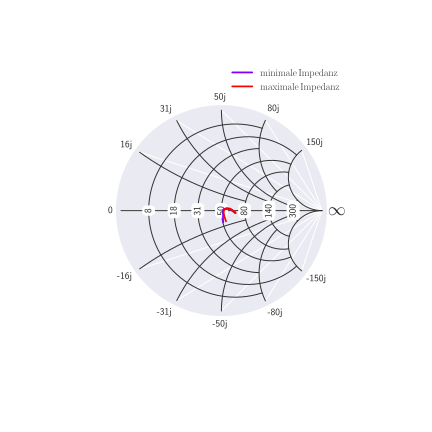
\includegraphics[width=0.9\textwidth]{data/images/messungen/input_Z_A8331}
    \caption{Inputimpedanz des A8331.}
    \label{fig:Z_in_A8331}
\end{center}
\end{figure}

Die Verstärkung sieht sehr gut aus wie Grafik \ref{fig:T_A8331} zeigt. Die Differenz zum soll ist stets kleiner als ein Dezibel. In Anbetracht des Umstandes, dass das Datasheet lediglich variable Verstärkungen auf 0.5 dB genau garantiert, ist weniger als 1 dB Abweichung extrem gut. Zudem muss berücksichtigt werden dass das Datasheet einen Verlust auf der externen Beschaltung von 0.4 dB zwischen den Pins LON und VOL sowie LOP und VOH spezifiziert.
Somit sieht die Kurve sogar noch viel besser aus.
Hier ist noch anzumerken, dass die Kurve um den Faktor $\frac{1}{a}$ und einen Faktor 2 korrigiert wurde. Der Faktor kommt daher dass das differentielle Signal nur die halbe Signalamplitude hat. 

\begin{figure}[H]
\begin{center}
    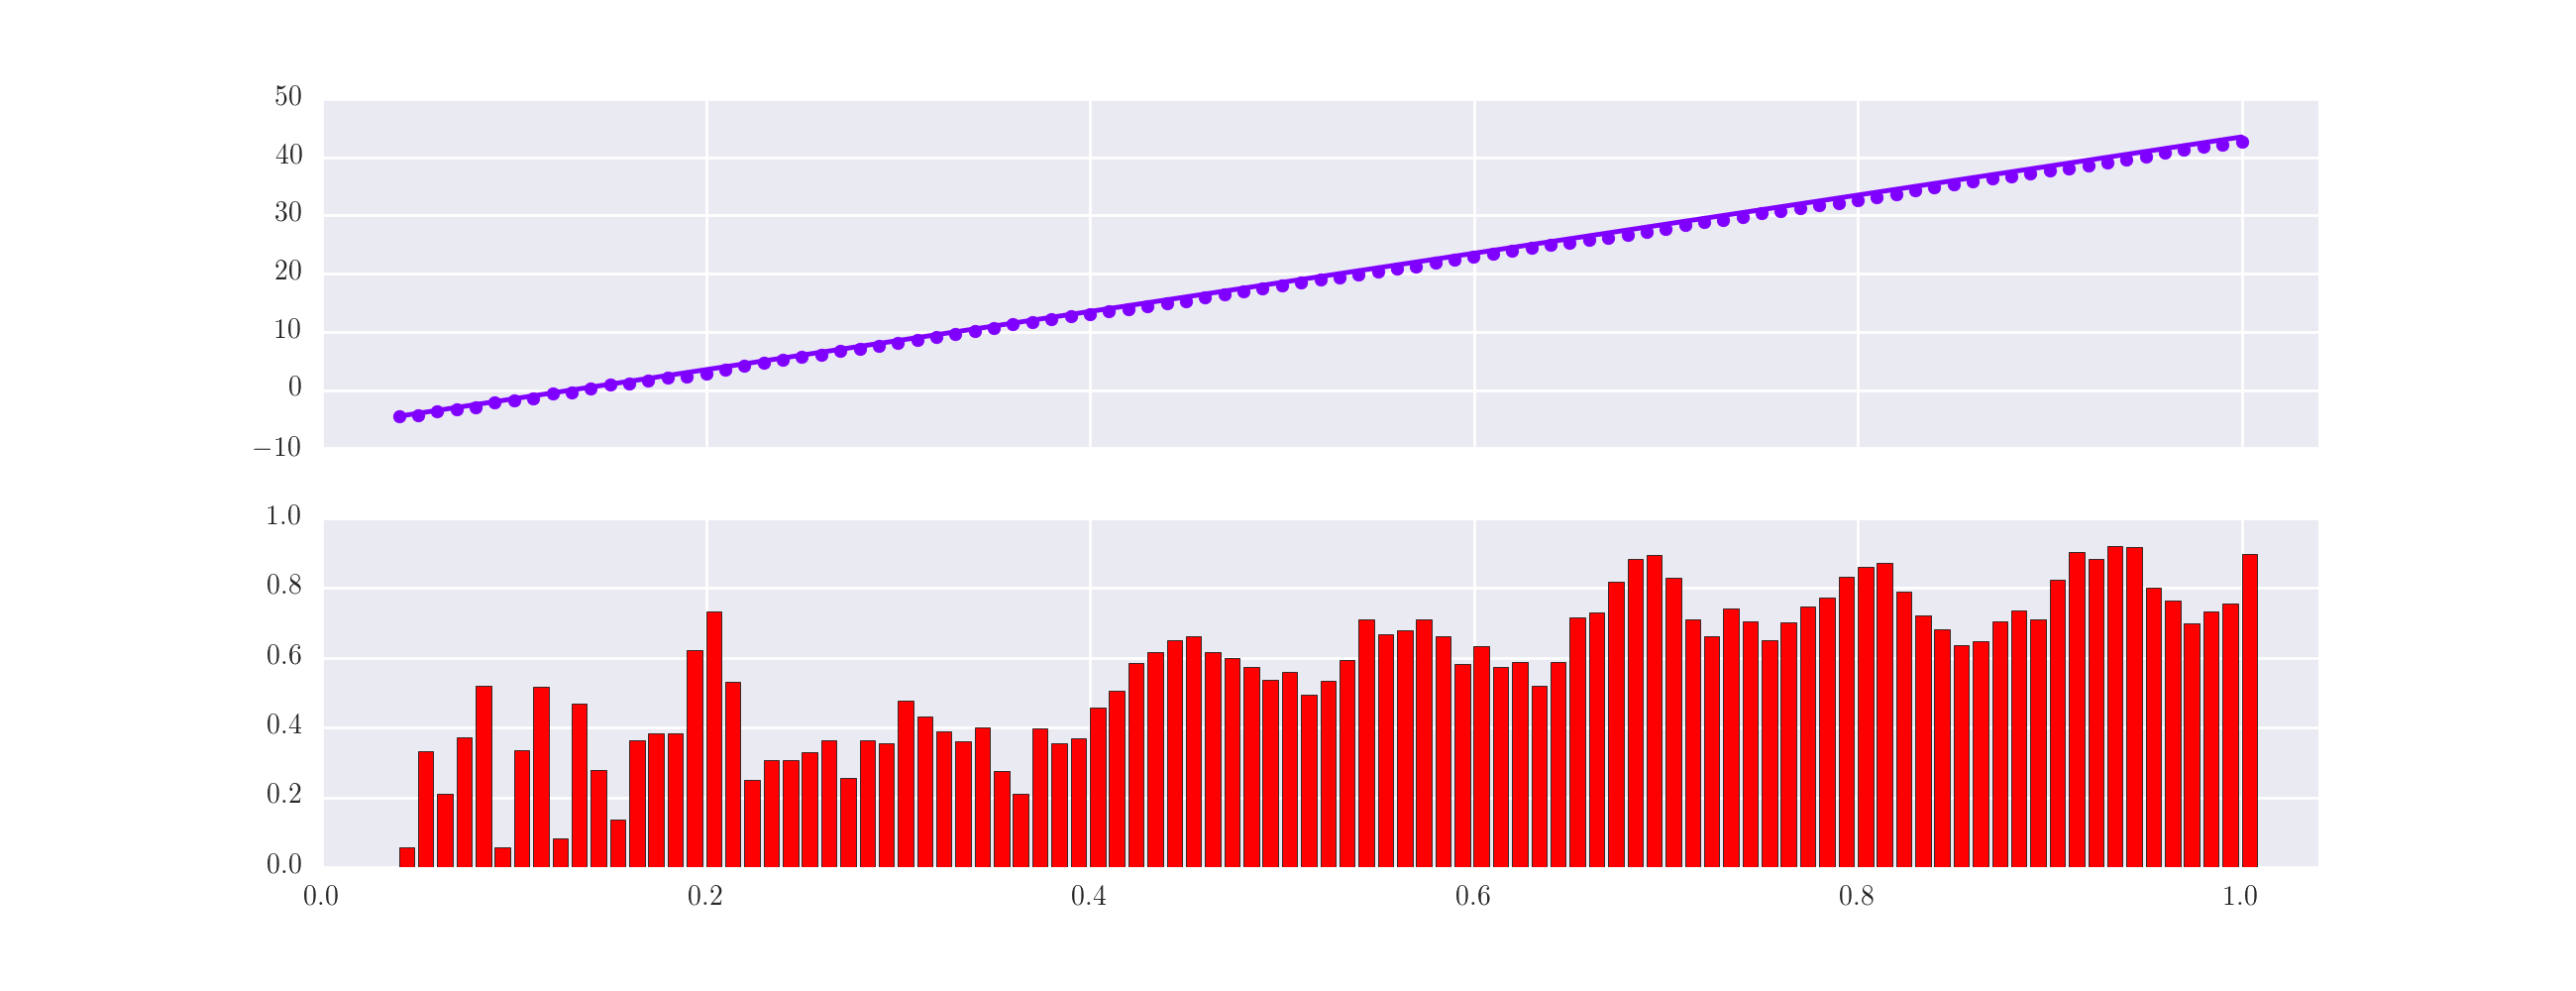
\includegraphics[width=0.9\textwidth]{data/images/messungen/vga_2016-12-22_30dBm_transmission2}
    \caption{Verstärkung des AD8331 gemittelt über einen 50 MHz Sweep. Ist und Soll gegenübergestellt. Zudem die Differenz zu jedem Wert.}
    \label{fig:T_A8331}
\end{center}
\end{figure}

Bei allen Messungen mit dem zweiten PCB ist der DAC nicht verbaut. Dies, da der Verdacht bestand, dass dieser viel Rauschen mit sich bringt, was nach der Erkenntniss dass der AD8331 auf dem ersten Board tatsächlich kaputt ist nicht mehr so wahrscheinlich ist. Er wurde durch eine externe Spannungsversorgung ersetzt. In weiteren Versuchen soll dieser natürlich noch genau evaluiert werden.

\subsubsection*{ISL55210}

Da die Messungen so gut herauskamen wurde angenommen dass somit der AD8331 als Input für weitere Messungen am ISL55210 verwendet werden kann, um weiterhin auf einen Balun verzichten zu können. Mit einem twisted Pair wurden die beiden Stufen also verbunden. so kann zwar die Inputimpedanz des ISL55210 zwar nicht mehr gemessen werden, hier reichte die Transmission jedoch völlig.

Im Plot \ref{fig:T_broken_ISL55210} sieht man das Verhalten des ISL55210. Sehr unschön. Es gibt aber drei interessante Dinge zu sehen.
Erstens stimmen die gemessenen Verstärkungen über den Frequenzsweep gemittelt gut mit dem Datasheet überein wie man in Grafik \ref{fig:T_broken_mean_ISL55210} sieht.

\begin{figure}[H]
\begin{center}
    \includegraphics[width=0.9\textwidth]{data/images/messungen/vga_lna_2016-12-22_50dBm_20dB_transmission3}
    \caption{Verstärkung des AD8331 und ISL55210 50 MHz Sweep bei 10 verschiedenen Verstärkungen.}
    \label{fig:T_broken_ISL55210}
\end{center}
\end{figure}

\begin{figure}[H]
\begin{center}
    \includegraphics[width=0.9\textwidth]{data/images/messungen/vga_lna_2016-12-22_50dBm_transmission2}
    \caption{Verstärkung des AD8331 und ISL55210 gemittelt über einen 50 MHz Sweep. Ist und Soll gegenübergestellt. Zudem die Differenz zu jedem Wert.}
    \label{fig:T_broken_mean_ISL55210}
\end{center}
\end{figure}

Dies kann ein Zufall sein. Was aber viel interessanter ist, dass die Kurve zwar sehr komisch ausschaut, aber überhaupt nicht wie jene, welche beim Vorgängerprojekt gemessen wurde, wie man unschwer in Grafik \ref{fig:ganzes_system_vorganger} erkennen kann.

\begin{figure}[H]
\begin{center}
    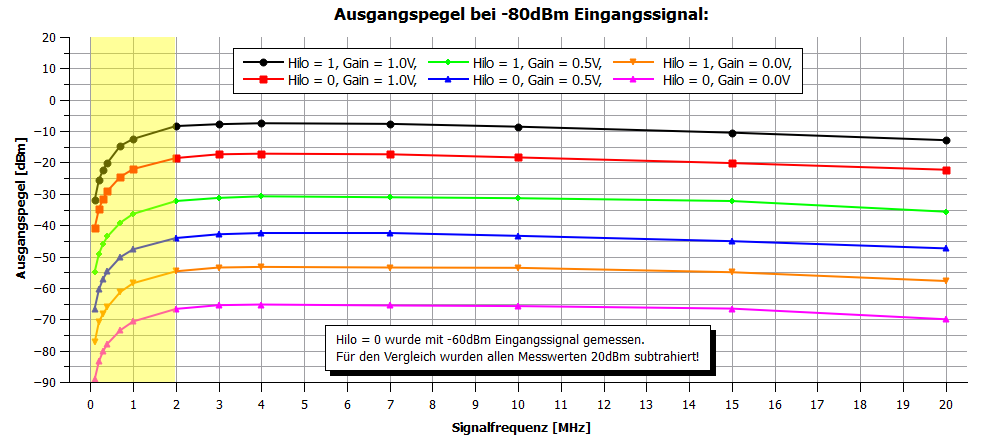
\includegraphics[width=0.9\textwidth]{data/images/ganzes_system_vorganger}
    \caption{Verstärkung des AD8331 und ISL55210. Gemessen im Vorgängerprojekt.}
    \label{fig:ganzes_system_vorganger}
\end{center}
\end{figure}

Bei dieser Kurve gibt es einen Unerwarteten Abfall bei 2 MHz abwärts, was in der Vorgängerarbeit auf das aktive Impedanzmatching geschoben wurde. Dieses Verhalten konnte in den gemachten Messungen nicht nachvollzogen werden. Im Gegenteil, es wird ein starker Anstieg gemessen in diesem Bereich.

Ein dritter Punkt ist, dass der Verstärker einen unerwarteten Abfall hat je höher die Frequenz ist. Laut Datasheet sollte der Verstärker locker bis 100MHz um 28 dB verstärken. Die Kurve müsste relativ gerade ausfallen. Erst war der Gedanke da, dass es nur ein Fehle rin diesem Projekt ist. Wie sich aber zeigt bestand dieses Verhalten schon im Vorgängerprojekt, wurde jedoch nicht explizit bemerkt oder wenigstens erwähnt. 